\section{String Matching Using Hashing and Rabin-Karp Algorithm}

\paragraph{
    We will go through an algorithm called the Rabin-Karp Algorithm which is a typical example of string matching. 
    The main idea is to use hashing to find the pattern in a string.\\
    But first, what is string matching exactly?\\
    Well, we want to know whether a given pattern is in a string or not, for example, does $p$ of size $m$ occur in 
    string $s$ of size $n$.\\
}

\begin{figure}[H]
    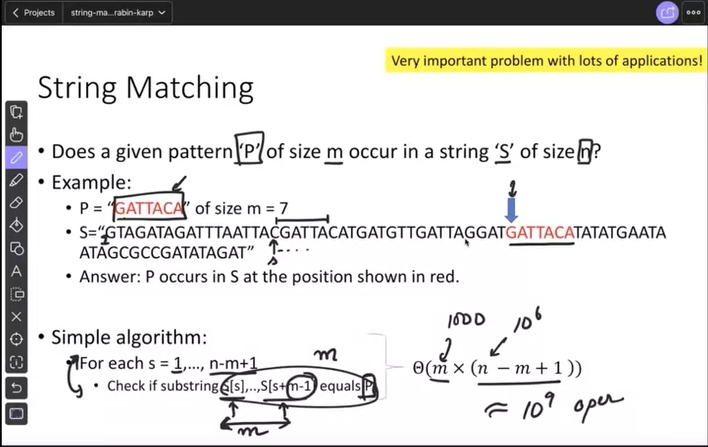
\includegraphics[width=\textwidth]{stringmatching.png}
\end{figure}

\paragraph{
    We can use a simple algorithm to solve the problem.\\
    First compute $r=h(p)$;\\
    Then for each $s = 1, 2, \ldots, n-m+1$, check if $s[1], s[2], \ldots, s[m]$ has the same hash value as $p$.\\
    The total running time of it is $\theta(m*(n-m+1))$.\\
    This is just a brute force method. Now we need to speed up the process.\\
    We can try to use hash functions to hash the pattern and the string.\\
}

\begin{figure}[H]
    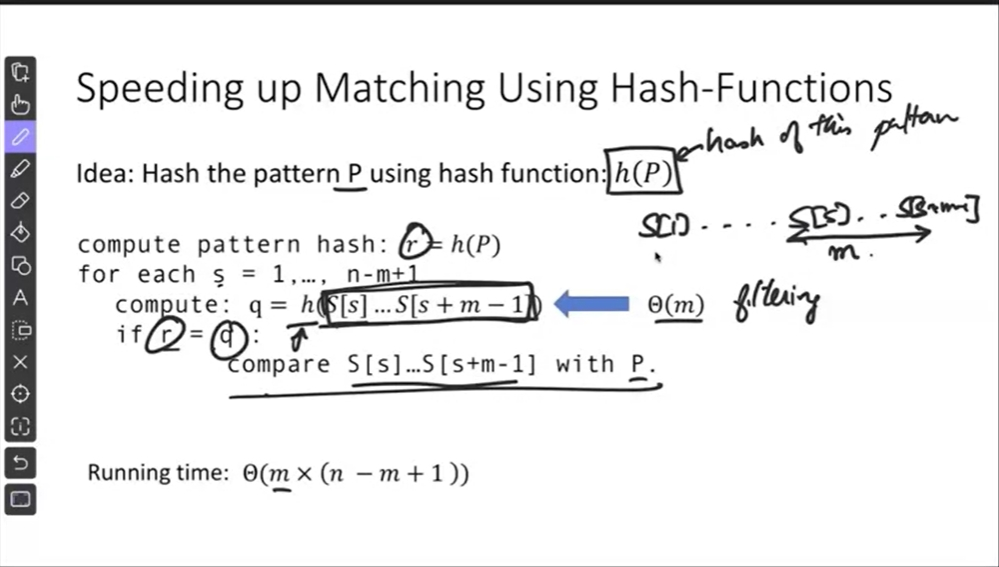
\includegraphics[width=\textwidth]{stringmatchingusinghash.png}
\end{figure}

\paragraph{
    We need to randomly choose a prime number in order to perform the rolling hash function.\\
    The main advantage of the rolling hash function is that it can hash the string in $O(1)$ time complexity.\\
    The idea is that when conducting hashes on different element $S$, for $S = 1, 2, \ldots, n$, 
    we can use the previous hash value to calculate the new hash value.\\
    $h(s[i], s[i+1], \ldots, s[i+m-1]) = h(s[i], s[i+1], \ldots, s[i+m-2]) * p + s[i+m-1]$.\\
    $h(s[i+1], s[i+2], \ldots, s[i+m]) = (h(s[i], s[i+1], \ldots, s[i+m-2]) - s[i]*p^{m-1})*p + s[i+m]$.\\
    Which equals to $p * h(s[i], s[i+1], \ldots, s[i+m-2]) + s[i+m-1]$.\\
    That is to say, the new hash value is the previous hash value times $p$ plus the new element.\\
    Using the rolling hash function mechanism, the worst case running time will still be $\theta(m*(n-m+1))$.\\
    But the average running time will be $\theta(n+m)$ when the function collision is low.\\
}

\begin{figure}[H]
    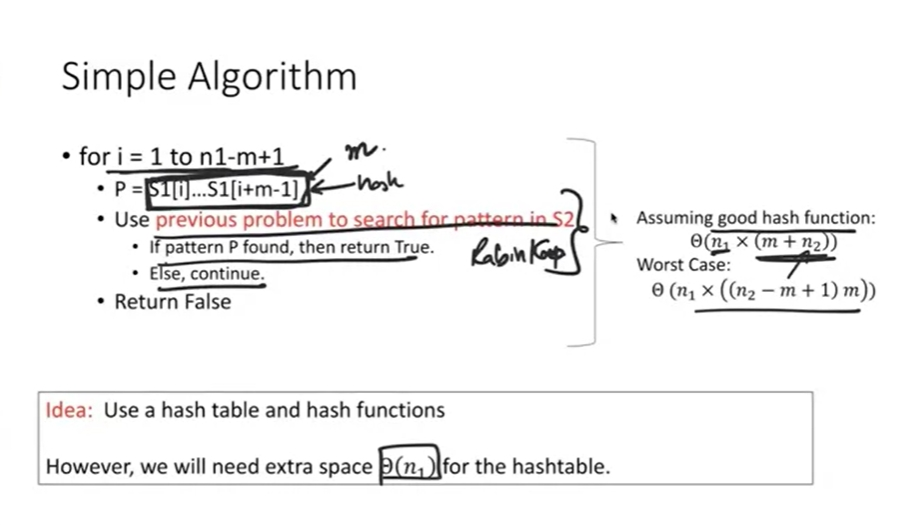
\includegraphics[width=\textwidth]{stringmatchingproblem2simplealgo.png}
\end{figure}

\paragraph{
    Instead of taking each pattern and comparing one by one, we can also hash all the pattern and store them in a hashtable.\\
    Then we will hash the string and compare the hash value with the hashtable.\\
    At first, we need to use the rolling hash of string 1, a.k.a. $h(s[i], s[i+1], \ldots, s[i+m-1])$.\\
    Then we will insert the `key/value` pair into the hashtable.\\
    After these steps, we will begin to hash string 2 by computing the rolling hash 
    $r_j= h(s_2(j), s_2(j+1), \ldots, s_2(j+m-1))$.\\
    Then we will check if $r_j$ is in the hashtable. If $r_j$ is in the hashtable, we will compare the pattern with the string.\\
    The running time of the above algorithm is $\theta(n+m)$.\\
}

\begin{figure}[H]
    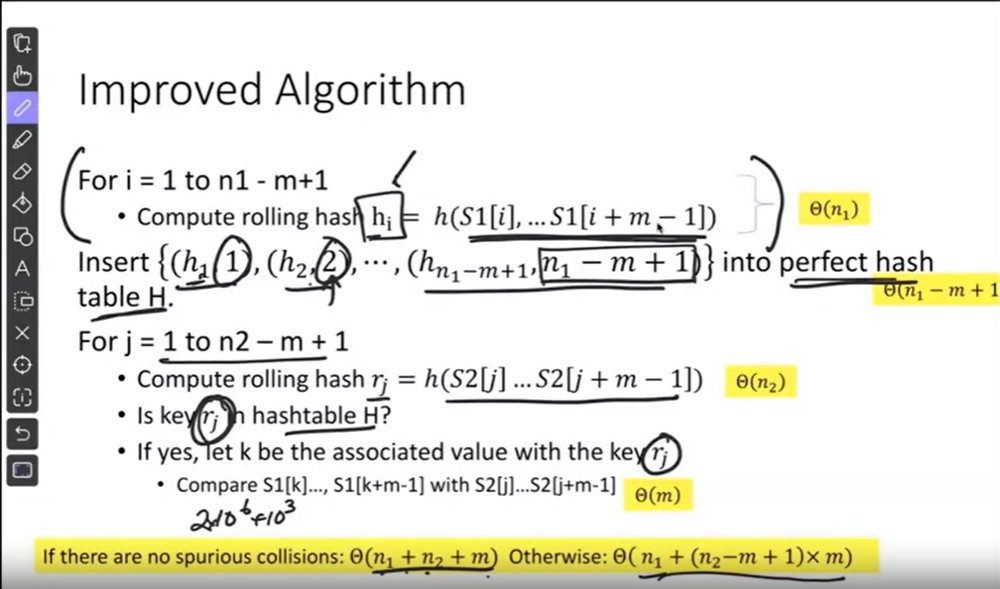
\includegraphics[width=\textwidth]{stringmatchingproblem2improvedalgo.png}
\end{figure}